\documentclass[a4paper]{jsarticle}
\usepackage[dvipdfmx, hiresbb]{graphicx}
\usepackage{booktabs}
\usepackage{macros}

\begin{document}
\title{第2章 \\ Sites and Topoi}
\author{七条彰紀}
\maketitle
\tableofcontents
\vspace{10pt}

\section{Motivation.}
scheme, stack等には以下のような包含関係がある.
\[\xymatrix{
    {} & \text{Algebraic Stack} \ar@{^{(}->}[r]& \text{Stack} \ar@{^{(}->}[r]& \text{Presheaf of Grupoids} \\
    \text{Scheme} \ar@{^{(}->}[r]\ar@{^{(}->}[ru]& \text{Algebraic Space} \ar@{^{(}->}[r]\ar@{^{(}->}[u]&
        \text{Space} \ar@{^{(}->}[r]\ar@{^{(}->}[u]& \text{Presheaf of Sets} \ar@{^{(}->}[u]
}\]
最終的にセミナーを通じて我々が定義したいのはalgebraic stackであるが,
今回はそれよりも定義が簡素な``space"を定義する.
先にspaceの定義文を示そう.

\begin{Def}[Space, \cite{GomezAS} p.26]
    $S$ :: schemeとする.
    Space over $S$ (or $S$-space)とは,
    big etale site over $S$上にある,集合のsheafである.
\end{Def}
ここに現れる``big etale site"と``big etale site上のsheaf"を以下で定義する.
さらにsheafの射について幾つか定義をすれば,
algebraic spaceまで定義できる.

定義だけではspaceのlocalは性質を調べる手段がないため,
次回は「高次版のsheafの貼り合わせ」と呼べる``Descent theory"を学ぶ.

\section{Sites.}

\subsection{Definitions.}
以下で導入するGrothendieck topologyは,
「Sheafを定義するのに必要な位相空間の定義を抽出し,圏論的に一般化したもの」である.
$X$ :: toplological spaceとし,sheaf on $X$の定義を見なおしてみよう.
すると,sheaf on  $X$は次に挙げるもののみを用いて定義されていると分かる.
\begin{enumerate}
    \item $X$の開部分集合と包含写像が成す圏.
    \item 開部分集合$U \subseteq X$のopen covering.
    \item 同じく$U$のopen covering :: $\{U_i\}_i$が与えられたときの族$\{ U_i \cap U_j \}_{i,j}$
\end{enumerate}
そこで次のように定義する.

\begin{Def}[Grothendieck Topology]
    $\cat{C}$ :: cateogoryについて,
    $\cat{C}$上のGrohendieck topologyは
    任意の$X \in \cat{C}$に
    $\cat{C}$の射の集まり$\{X_i \to X\}_{i \in I}$の集まり(collection of collections)を
    対応させる$\Cov$で構成される.
    さらに,$\Cov$は以下を満たすように要請される.
    \begin{enumerate}[label=(\alph*)]
        \item
            $X' \to X$ :: isoならば$\{X' \to X\} \in \Cov(X)$.
        \item
            $\{U_i \to U\} \in \Cov(U), V \to U \in \cat{C}$について,
            $\{U_i \times_U V \to V\} \in \Cov(V)$.
        \item
            $\{U_i \to U\}_i \in \Cov(U)$をとり,
            さらに各$i$について$\{V_{i,j} \to U_i\}_j \in \Cov(U_i)$をとる. \mbox{}\\
            この時,合成も$\Cov$に入っている : $\{V_{i,j} \to U_i \to U\}_{i,j} \in \Cov(U)$.
    \end{enumerate}
\end{Def}

\begin{Remark}
    ここで「集合」ではなく「集まり」という言葉を用いたのは,
    これらが集合ではない可能性があるからである.
    この問題(圏論でもしばしば現れる)を取り扱うためには,
    $2$つの解決策がある.
    $1$つ目はGrothendieckの宇宙公理UをZFC公理系に加えたZFCU公理系で議論を行うことである.
    もう$1$つは真のクラスを扱えるNBG公理系で議論を行うことである.
    
    後者の方針を採用する場合は,
    Grothendieck topologyの定義で現れた「集まりの集まり」という言葉に注意が必要である.
    というのも,たとえNBG公理系でも,
    真のクラスを要素に持つ真のクラスは許されていないからである.
    この問題を解決するには以下のように$\Cov$を定義すれば良い
    (以下のように書き換えれば良いという事がわかれば十分なので,
    実際に以下の定義を採用することはない):

        全ての$U \in \cat{C}$について$\Cov(U)$はcodomainが$U$である射のクラスである.
        任意の要素$[ V \to U ] \in \Cov(U)$について
        この要素を含む$\Cov(U)$の部分クラス$\{U_i \to U\}_i \subset \Cov(U)$が存在し,
        以下が成立する.
        (以下略).
\end{Remark}

$\Cov$の元には大抵,以下の条件が課される.
\begin{Def}[(Jointly) Surjective Family]
    ある圏の射の集まり$\{U_i \to U\}_i$について,
    \[ \bigsqcup_i U_i \to U \]がsurjectiveである時,
    (同値な条件として,
    $\im (U_i \to U)$のset-theoritic unionが$U$に等しい時,)
    この集まり$\{U_i \to U\}$を(jointly) surjective familyという.
\end{Def}

\begin{Def}[Site]
    圏$\cat{C}$と$\cat{C}$上のGrothendieck topology :: $\Cov$の組をsiteと呼ぶ.
    siteに対し,その部分である圏をthe underlying categoryと呼ぶ.
    しばしば$\Cov$を略して$\cat{C}$のみでsiteを表す.
\end{Def}

\begin{Def}[Localized Site.]
    site :: $\cat{C}$と$X \in \cat{C}$について,
    localized site :: $\cat{C}/X$を以下のように定義する.

    $\cat{C}/X$のunderlying categoryはslice cageory :: $\cat{C}/X$である.
    したがって対象は$\cat{C}$内の$X$への射である.
    Grothendieck topology :: $\Cov$は,
    \[
        \{ [U_i \to X] \to [U \to X] \}_i \in \Cov([U \to X])
        \implies \{U_i \to U\} \in \Cov(U).
    \]
    のように定められる.
\end{Def}

\begin{Def}[Diagrams (or Comma Site).]
    $\Delta$ :: category, $\cat{C}$ :: site, 
    $F \colon \Delta^{op} \to \cat{C}$ :: functorとする.
    この時site :: $\cat{C}_F$を以下のように定める.

    まずundrelying categoryは$(\id[\cat{C}] \downarrow F)$である.
    したがって対象は$X \to F(\delta) \ (\delta \in \Delta)$である.
    $\Cov$は以下のように定める.
    \[
        \left\{
        \vcenter{
        \xymatrix@R=8pt{
            X'_i \ar[d]\ar[r]^-{f_i^{\flat}}& X \ar[d]\\
            F(\delta_i) \ar[r]_-{F(f_i)}& F(\delta)
        }}
        \right\} \in \Cov([X \to F(\delta)])
        \implies
        f_i \colon \delta \to \delta_i \text{ :: iso. and }
        \{f_i^{\flat} \colon X'_i \to X \} \in \Cov(X).
    \]
\end{Def}

\begin{Def}[Continuous Functor.]
    $\cat{C}, \cat{C}'$ :: sitesとする.
    $f \colon \cat{C} \to \cat{C}'$ :: functorがcontinuousとは,
    以下の$2$つが成立すること:
    \begin{enumerate}
        \item 
        任意の$X \in \cat{C}$と$\{U_i \to X\}_i \in \Cov_{\cat{C}}(X)$について,
        \[ \{ f(U_i) \to f(X) \}_i \in \Cov_{\cat{C}'}(f(X)) \]となる.

        \item
        $\cat{C}$の任意の射$X_1 \to Y, X_2 \to Y$について,
        fiber product :: $X_1 \times_Y X_2$が$\cat{C}$に存在するならば,
        \[ f(X_1 \times_Y X_2) \iso f(X_1) \times_{f(Y)} f(X_2). \]
    \end{enumerate}
\end{Def}

\begin{Remark}
    後に示すように,
    continuous functorはよくあるケースでcategory of sheaves on siteの間の関手を誘導する.
    これはschemeの間のcontinuous mapが
    category of sheaves on schemeの間の
    関手(e.g. inverse image functor, direct image functor)を定めるのと同じである.
\end{Remark}

\subsection{Examples.}

\subsubsection{Site.}
\begin{Example}[Classical topology.]
    $X$ :: topological spaceとし,
    $O(X)$を以下のような圏とする.
    \begin{description}[labelindent=5mm]
        \item[対象] $X$の開集合.
        \item[射] 包含射.
    \end{description}
    この時,$U \in O(X)$のcovering :: $\Cov(U)$を,
    $U$への包含射のみから成るjointly surjective familyの集合
    \footnote{ 包含射の個数は高々$2^{\#X}$以下の濃度なので,familyの集まりは集合. }
    とする.

    以上で定まるsite :: $(O(X), \Cov)$は
    通常のtopologyをGrothendieck topologyの枠組の中で再現している.
\end{Example}

以下で主に用いるのは,
$\cat{C}$がslice category :: $\Sch/X \ (X \in \Sch)$の部分圏であるようなsiteである.
$X \in \Sch$に対して,
このようなsiteはunderlying category ($\subset \Sch/X$)と
Grothendieck topology ($\Cov$)からなるから, 
以下の図の(a) $U \to X$, (b) $U_i \to U$がどのようなものであるか定めれば定義できる.
\begin{center}
     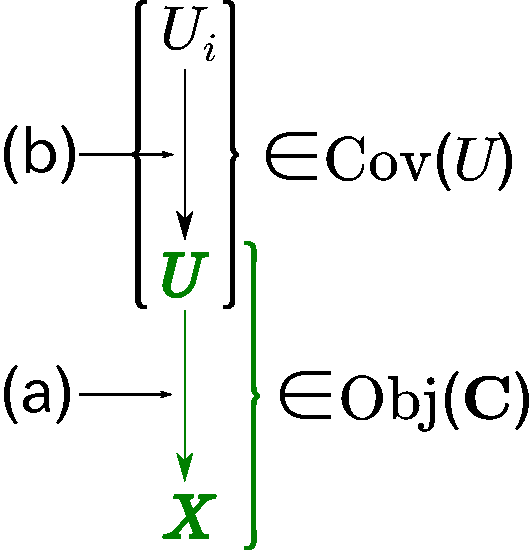
\includegraphics[width=5cm]{./images/site.pdf}
\end{center}
すなわち,以下の未完成な定義文をテンプレートとする,一連の定義文の群がある.
\begin{Def}[$***$ site]
    $X$ :: schemeについて,
    圏$\cat{C}$を以下で定める.
    \begin{description}[labelindent=5mm]
        \item[対象] (a)である射$U \to X$.
        \item[射]   二つの対象の間の射$[U \to X] \to [U' \to X]$は,$X$-morphism :: $U \to U'$.
    \end{description}
    $[U \to X] \in \cat{C}$に対して,
    $\Cov(U)$を(b)である射の集まり$\{U_i \to U\}_i$であって
    jointly surjective familyであるものの集まりとする.

    以上の$\cat{C}$と$\Cov$からなるsiteを $***$ site of $X$と呼ぶ.
\end{Def}

Grothendieck topologyの定義から分かるとおり,
性質(b)がstable under base change \& compositionであれば,
以上のテンプレートはsiteの定義文と成る.

\begin{samepage}
\begin{Def}
    以上の定義文テンプレートを用いて,(a), (b)と各siteの定義を以下のように対応させる.
    (a)が``--"とある箇所は「$\Sch/X$の任意の射」を意味する.
    さらに,``open inclusion"はZariski開集合の間にある包含射のことである
    (したがってsmall Zariski siteのunderlying categoryにはZariski開集合しか無い).

\begin{table}[ht]
\begin{tabular}{c|lllllll}
\toprule
    $***$ & small Zariski  & big Zariski    & small etale & big etale\\ \midrule
    (a)   & open immersion & --             & etale       & --       \\
    (b)   & open immersion & open immersion& etale       & etale    \\ \hline \hline
    $***$ & lisse-etale & smooth & fppf                                   & fpqc                  \\ \midrule
    (a)   & smooth      & smooth & --                                     & --                    \\
    (b)   & etale       & smooth & flat\&locally of finite presentation & flat\&quasi-compact \\ \bottomrule
\end{tabular}
\end{table}

    図の再掲:
    \begin{center}
         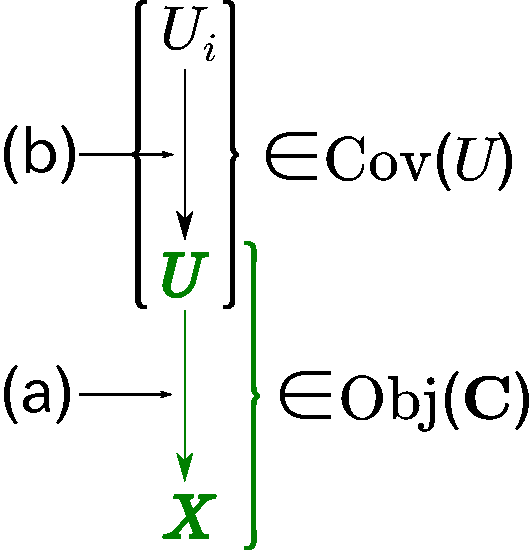
\includegraphics[width=5cm]{./images/site.pdf}
    \end{center}
\end{Def}
\end{samepage}

\begin{Remark}
``fppf"は
``fid\`{e}lement plate de pr\'{e}sentation finie"(仏語)すなわち
``faithfully flat and of finite presentation"の略である.
flat\& locally of finite presentationならば実際にこのように成る.
同様に``fpqc"は``fid\`{e}lement plat et quasi-compact"(仏語)すなわち
``faithfully flat and quasi-compact"の略である.
\end{Remark}

\begin{Def}
    $***$ site of $X$の記号を以下のように定める.
\begin{table}[ht]
\begin{tabular}{c|lllllllll@{}}
    \toprule
    $***$ & small Zariski     & big Zariski       & small etale      & big etale\\ \midrule
    名前    & $\mathrm{Zar}(X)$ & $\mathrm{ZAR}(X)$ & $\mathrm{Et}(X)$ & $\mathrm{ET}(X)$ \\ \hline \hline
    $***$ & lisse-etale         & smooth           & fppf               & fpqc               \\ \midrule
    名前    & $\mathrm{Lis\mdash Et}(X)$ & $\mathrm{Sm}(X)$ & $\mathrm{Fppf}(X)$ & $\mathrm{Fpqc}(X)$ \\ \bottomrule
\end{tabular}
\end{table}

    \cite{StacksProj}ではbig Zariski site of $X$を$(\Sch/X)_{Zariski}$などと書く.
\end{Def}


\subsubsection{Continuous Functor.}
\begin{Example}
    $X, X'$ :: topological spaceについて,
    $O(X), O(X')$ :: classical site,
    $f \colon X \to X'$ ::continuous mapとする.
    この時,$f^{-1} \colon O(X') \to O(X)$ :: continuous functor.
    ($f$は必ずしもcontinuous functorでないことに注意.)
\end{Example}

\begin{Remark}
    $f \colon \cat{C} \to \cat{C}'$ :: functor between sitesが
    continuousであるための条件を再掲する.
    \begin{enumerate}
        \item 
        任意の$X \in \cat{C}$と$\{U_i \to X\}_i \in \Cov_{\cat{C}}(X)$について,
        \[ \{ f(U_i) \to f(X) \}_i \in \Cov_{\cat{C}'}(f(X)) \]となる.

        \item
        $\cat{C}$の任意の射$X_1 \to Y, X_2 \to Y$について,
        fiber product :: $X_1 \times_Y X_2$が$\cat{C}$に存在するならば,
        \[ f(X_1 \times_Y X_2) \iso f(X_1) \times_{f(Y)} f(X_2). \]
    \end{enumerate}
    
    例と照らし合わせると,
    $1$つめの条件は$f^{-1}$が開集合を開集合に写すことに対応し,
    $2$つめの条件は$f^{-1}$が$\cap$と交換することと対応する.
\end{Remark}

\begin{Example}
    従属関係
    \[ \text{open immersion} \implies \text{etale} \implies \text{fppf} \]
    があるから,
    inclusion map :: $\mathrm{Zar}(X) \inclmap \mathrm{ET}(X) \inclmap \mathrm{Fppf}(X)$
    はそれぞれcontinuous.
\end{Example}

\begin{Example}
    flat morphism :: $f \colon X \to Y$をとり,
    $f$によるpullback functorを$P_{f}$とする.
    (TODO: 要確認.)
\end{Example}

\section{Sheaves.}
\subsection{Definitions.}
\begin{Def}[Sheaf, Topos, Morphism of Topoi.]
    \begin{myenum}
    \item
    site :: $S$上のpresheafとは,
    functor :: $\shF \colon S^{op} \to \Sets$のことである.

    \item
    射影$U \times_B V \to U$をpresheaf :: $\shF$で写した射を$\res_{U}^{U \times_B V}$と書く.

    \item
    presheaf on $S$ :: $\shF$がsheafであるとは,
    以下の図式がequalizer diagramであるということ.
    \[\xymatrix{
        \shF(U) \ar[r]& \prod_{i \in I} \shF(U_i)
            \ar@<1mm>[r]\ar@<-1mm>[r]& \prod_{(i,j) \in I \times I} \shF(U_i \times_U U_j)
    }\]
    ここで右の並行射は$\res_{U_i}^{U_i \times U_j}, \res_{U_j}^{U_i \times U_j}$である.

    \item
    Site :: $S$上の,
    圏$\cat{C}(=\Sets, \mathrm{Rings}, \mathrm{AbGrp}, \dots)$への
    presheafの圏を$\PSh(S, \cat{C})$,sheafの圏を$\Sh(S, \cat{C})$と書く.
    $\cat{C}=\Sets$の場合は略して$\Sh(S), \PSh(S)$と書く.

    \item
    morphism of shaeves :: $\shF \to \shF'$とは,
    natural transformationのことである.

    \item
    $T$ :: categoryがtoposであるとは,
    category of sheaves of sets on a siteと圏同値であるということである.

    \item
    $T, T'$ :: topoiとする.
    morphism of topoi :: $f \colon T \to T'$とは,
    以下の$3$つの射($2$ functor and $1$ isomorphism.)からなる.
    \[
        f_* \colon T \to T', \quad f^* \colon T' \to T,
        \quad \phi \colon \Hom_{T}(f^*(-), -) \isomap \Hom_{T'}(-. f_*(-)).
    \]
    \end{myenum}
\end{Def}

\begin{Remark}
    上で定義したsheaf of setsと同様に,
    sheaf of abelian groups, sheaf of rings, ...が定義できる.
    これらはそれぞれsheaf of setsの圏 :: $\Sh(\cat{C}, \Sets)$における
    abelian group objects, ring objects, ...と定義される.
\end{Remark}

\begin{Remark}
    ``Topos"はギリシャ語で「場(place)」を意味する.
    ギリシャ語なので複数形は``topoi".

    $X$ :: schemeについて,
    $X$に関するtoposを$X_{et}, X_{ET}, \dots$などと書く.
    著者(例えば\cite{StacksProj})によっては
    これらの記号を$\Sch/X$をunderlying catgoryとするsiteに用いる.
    しかし``Grothendieck’s insight is that the basic object of study is the topos, not the site."
    (M.Olsson ``Stacks")というということから,
    toposにsiteより簡単な記号を与えるのは理解できることである.
\end{Remark}

\begin{Def}[Direct Image Functor.]
    $f \colon \cat{C} \to \cat{C}'$をfunctor of sitesとする.
    この時,$F \in \PSh(\cat{C})$について
    \[ f_*F(-):=F(f(-)) \]
    とおくと,$f_* F \in \PSh(\cat{C}')$が得られる.
    $f$ :: continuous functorならば,
    $\shF \in \Sh(\cat{C})$に対し
    同様にして$f_*\shF \in \Sh(\cat{C}')$が得られる.
\end{Def}

\begin{Def}[Ringed Topos.]
\begin{myenum}
    \item
    $T$ :: toposと$T$のring object :: $\Lambda$を合わせてringed toposと呼ぶ.

    \item
    morphism of ringed topoi :: $(f, f^{\#}) \colon (T, \Lambda) \to (T', \Lambda')$は,
    \begin{itemize}
        \item morphism of topoi :: $f=(f_*, f^*, \phi) \colon T \to T'$と,
        \item morphism of ring in $T'$ :: $f^{\#} \colon \Lambda' \to f_* \Lambda$
    \end{itemize}
    の組である.
\end{myenum}
\end{Def}

\subsection{Examples.}
\begin{Example}
    $X$ :: schemeと,
    $\Sch/X$の部分圏をunderlying categoryとするsite :: $\cat{C}$(e.g. small/big Zariski site)について,
    $\ftor{X}(-)=\Hom_{\cat{C}}(-, X)$で
    functor :: $\ftor{X} \colon \cat{C} \to \Sets$を定める.
    この時,$\ftor{X}$ :: presheaf on $\cat{C}$.
    特に,後に示すとおり,
    fppf toplogyより荒い位相(e.g. Zariski, smooth, etale, ...)でsheafとなる.
\end{Example}

\begin{Example}[Constant (Pre)sheaf.]
    $\cat{C}$ :: siteとし,
    以下のようにpresheaf on $\cat{C}$ :: $\shF$を定める.
    \[ \shF \colon \emptyset \neq U \mapsto \R, \qquad \emptyset \mapsto \{0\}.  \]
    constant presheaf on a schemeがsheafでないのと全く同じ理由で,
    この$\shF$はsheafでない.
    具体的には$U \in \cat{C}$が連結でないschemeならば,
    $U_1 \sqcup U_2=U$なるcoveringを取ると,
    定義にあるdiagramがequalizer diagramにならない.
\end{Example}

\begin{Example}
    $S$ :: schemeについて,
    $\Sch/S$上のpresheafを
    \[ \shO_S \colon [X \to S] \mapsto \Gamma(X, \shO_X) \]
    で定める.
    このsheafは``structure sheaf of $S$"と呼ばれ,$\ftor{\affine^1_S}$と同型.
\end{Example}

\subsection{Propositions.}
\begin{Thm}\label{thm:Shff}
    $\cat{C}$ :: siteとする.
    忘却関手
    \[ \ftorFgt \colon \Sh(\cat{C}) \to \PSh(\cat{C}). \]
    はleft adjoint functor :: $\ftorSh$を持つ.
\end{Thm}
%% {{{
\begin{Remark}
    以下で述べる$\ftorSh$の構成は``plus construction"と呼ばれる.
    Kay Werndli ``Sheaves From Scratch" \S3.5ではetale bundleという物を用いた構成をしている.
\end{Remark}

証明のために幾つか定義しておく.

\begin{Def}[\cite{StacksProj}, Tag 00W1]
    $\shF \in \PSh(\cat{C})$と,
    $X \in \cat{C}$のcover :: $\covU=\{U_i \to X\} \in \Cov(X)$に対し,
    \[ H^0(\covU, \shF)=\text{equalizer of }\left[
        \vcenter{\xymatrix{
        \prod_{i \in I} \shF(U_i)
        \ar@<1mm>[r]^-{} \ar@<-1mm>[r]_-{}&
        \prod_{(i,j) \in I \times I} \shF(U_i \times_X U_j)
    }} \right] \]
    ここで二つの並行射は
    それぞれ$\res_{U_i}^{U_i \times U_j}, \res_{U_j}^{U_i \times U_j}$である.
    すなわち,ここにある並行射はsheafの定義にあるものである.
    このdiagramは圏$\Sets$の中のものなので,
    \textbf{index :: $I$が集合ならば}このequalizerは常に存在する.
    ($H^0$という記号は,これが$\shF$の$0$次\v{C}ech cohomologyであることによる.)
    
    直ちに分かるとおり,$\Cov(X)$は細分を射として圏を成し,
    $H^0(-, \shF)$は圏$\Cov(X)$から$\Sets$への反変関手である.
    $\shF^+$は
    \[ \shF^+(X)=\Colim_{\covU \in \Cov(X)} H^0(\covU, \shF)=\Colim(\Cov(X) \to^{H^0(-,\shF)} \Sets). \]
    と定義される
    \footnote
    {
        定義から,$s,t \in \shF^+(X)$が等しいとは,以下が成り立つこと:
        $s, t$へそれぞれ写る
        $(\tilde{s}_U)_{U \in \covU} \in H^0(\covU, \shF),
            (\tilde{t}_{V})_{V \in \covV} \in H^0(\covV, \shF)$
        が存在し,
        $\covU, \covV$の共通のある細分$\covW$において
        \[ (\tilde{s}_U|_{W})_{\covW \ni W \subseteq U \in \covU}
            =(\tilde{t}_{V}|_{W})_{\covW \ni W \subseteq V \in \covV} \]
        となる.
    }.
    任意の$\covU \in \Cov(X)$について,
    常に標準的全射$\iota_{\covU} \colon H^0(\covU, \shF) \to \shF^+(X)$が存在する.

    $H^0(\{\id[X] \colon X \to X\}, \shF)=\shF(X)$であり,
    しかも任意のcover of $X$は$\id[X]$の細分であるから,
    $X$毎に標準的な射$\theta \colon \shF(X) \to \shF^+(X)$が存在する.
    \[\begin{tikzcd}
            {} & \shF(X) \ar[r, dashed, "\theta"]\ar[rd, bend left=20] \ar[d]& \shF^+(X) \\
        \shF(X) \ar[r, phantom, "\in"]&
            \Big\{H^0(\covU, \shF) \ar[r]\ar[ru, bend right=10]&
            H^0(\covU', \shF) \Big\}_{\covU, \covU'}\ar[u]
    \end{tikzcd}\]
\end{Def}

\begin{Def}
    presheaf :: $\shP \in \PSh(\cat{C})$は以下を満たす時separatedであるという.
    \[ \Forall{X \in \cat{C}} \Forall{\{U_i \to X\}_i \in \Cov(X)}
        \shP(X) \to \prod_{i \in I} \shP(U_i)\text{ :: inj.} \]
\end{Def}

\begin{Lemma}[A]
    site :: $\cat{C}$, presheaf :: $\shF \in \PSh(\cat{C})$を考える.
    任意の$X \in \cat{C}, \covU \in \Cov(X), U_0 \in \covU$について,
    以下の図式は可換である.
    \[\begin{tikzcd}
        \shF^+(X) \ar[r, "\res_X^{U_0}"]& \shF^+(U_0) \\
        H^0(\covU, \shF) \ar[r, "\pr_{U_0}"']\ar[u, "\iota_{\covU}"]& \shF(U_0)\ar[u, "\theta"'] \\
        \prod_{U \in \covU} \shF(U) \ar[u, phantom, "\text{\rotatebox{-90}{$\subseteq$}}"]
    \end{tikzcd}\]
\end{Lemma}
\begin{proof}
    適当に$(\tilde{s}_U)_{U \in \covU} \in H^0(\covU, \shF)$をとり,
    $s=\iota_{\covU}\big((\tilde{s}_U)_{U \in \covU}\big) \in \shF^+(X)$とする.
    \[
    \xymatrix
    {
        s \ar[r]^-{\res_{X}^{U_0}}& s|_{U_0} \\
        (\tilde{s}_U)_{U \in \covU}
        \ar[u]\ar[r]^-{\prod \res_{U}^{U \times U_0}}\ar@/_5mm/[rd]_-{\pr_{U_0}}
        &(\tilde{s}_U|_{U \times U_0})_{U \in \covU} \ar[u]\\
            & \tilde{s}_{U_0}\ar@/_15mm/[uu]_-{\theta} \ar[u]^-{\prod \res_{U_0}^{U \times U_0}} 
    }
    \qquad \qquad
    \xymatrix
    {
        \shF^+(U) \ar[r]& \shF^+(U_0) \\
        H^0(\covU, \shF) \ar@{>->}[u]\ar[r]\ar@/_5mm/[rd]
            & H^0(\covU \times U_0, \shF) \ar@{>->}[u]\\
            & \shF(U_0) \ar@/_15mm/[uu]_-{\theta} \ar[u] 
    }
    \]
    $(\tilde{s}_U)_{U \in \covU}$から$(\tilde{s}_U|_{U \times U_0})_{U \in \covU}$への$2$本の射が
    一致するのは,$H^0(\covU, \shF)$の定義から従う
    \[ \tilde{s}_{U}|_{U \times U_0}=\tilde{s}_{U_0}|_{U \times U_0} \]
    が理由である.
\end{proof}

\begin{Lemma}[B]
    任意の$X \in \cat{C}$と$\covU, \covV \in \Cov(X)$に対し,
    $\covU, \covV$の共通の細分が存在する.
\end{Lemma}
\begin{proof}
    具体的に
    \[
        \covU \times \covV
        =\{ U \times V \to U \to X \mid U \in \covU, \covV \in \covV\}
        =\{ U \times V \to V \to X \mid U \in \covU, \covV \in \covV\}
    \]
    と取れば良い.
\end{proof}

\begin{Lemma}
    site :: $\cat{C}$, presheaf :: $\shF \in \PSh(\cat{C})$について
    以下が成り立つ.
    \begin{enumerate}[label=(\alph*)]
        \item $\shF^+$ :: separated. 
        \item $\shF^+$ :: sheaf if $\shF$ :: separated.
        \item $\theta \colon \shF \to \shF^+$ :: iso if $\shF$ :: sheaf.
        \item $\theta \colon \shF \to \shF^+$ :: universal,
    \end{enumerate}
\end{Lemma}
\begin{proof}
    \step{$\shF^+$ :: separated.}
    $X \in \cat{C}$をとり,$s, t \in \shF^+(X)$をとる.
    あるcover of $X$ :: $\covU \in \Cov(X)$について
    \[ \Forall{U \in \covU} s|_{U}=t|_{U} \]
    が成り立つと仮定して$s=t$を示す.
 
    まず,
    $\iota_{\covU'}\big( (\tilde{s}_{U'})_{U' \in \covU'} \big)=s$となる様に
    $\covU' \in \Cov(X)$と$(\tilde{s}_{U'}) \in H^0(\covU', \shF)$をとる.
    $\covU'$を必要に応じて更に細かくとれば,
    $t$についても同様の$(\tilde{t}_{U'}) \in H^0(\covU', \shF)$が存在するように出来る.
    さらに,$\covU'$を$\covU$の細分とする.
    
    この時,補題Aと$\covU'$が$\covU$の細分であることと仮定から
    \[ s|_{U'}=\theta(\tilde{s}_{U'})=\theta(\tilde{t}_{U'})=s|_{U'} \ (\in \shF^+(U')). \]
    したがって$\shF^+(U')$の定義から,
    各$U'$について以下のような条件を満たす$\covV_{U'} \in \covV(U')$が存在する:
    $(\tilde{s}'_{V})_{V \in \covV_{U'}},
        (\tilde{s}'_{V})_{V \in \covV_{U'}} \in H^0(\covV_{U'}, \shF)$であって
    \[
        \iota\big( (\tilde{s}'_{V})_{V \in \covV_{U'}} \big)=s|_{U'},\quad
        \iota\big( (\tilde{t}'_{V})_{V \in \covV_{U'}} \big)=t|_{U'}
    \]
    となるならば
    $(\tilde{s}'_{V})_{V \in \covV_{U'}}=(\tilde{t}'_{V})_{V \in \covV_{U'}}$
    となる.
    これら$\covV_{U'}$達を束ねて
    $\covU'$の細分$\covV=\{V \to U' \to U \to X\} \in \Cov(X)$を得る.
    $(\tilde{s}_{U'}), (\tilde{t}_{U'})$も細分して
    \[
        \tilde{s}=(\tilde{s}_{U'}|_{V})_{\covV \ni V \subseteq U' \in \covU'},\ 
        \tilde{t}=(\tilde{t}_{U'}|_{V})_{\covV \ni V \subseteq U' \in \covU'}
        \in H^0(\covU^2, \shF)
    \]
    を得る.
    
    以上の議論から,各$U'$について
    \[
        \Forall{ U' \in \covU' } \Forall{ V \in \covV }
        V \subseteq U' \implies
        \tilde{s}'_{V}=\tilde{t}'_{V} \in H^0(\covV, \shF).
    \]
    $\covV$は$\covU'$の細分だから,
    これは結局$\tilde{s}=\tilde{t}$ということである.
    さらに,$\tilde{s}, \tilde{t}$は
    $(\tilde{s}_{U'})_{U' \in \covU'}, (\tilde{t}_{U'})_{U' \in \covU'}$の細分
    \footnote{ 被覆の細分に合わせた呼び方である.多分,$H^0(-, \shF)$の元に用いるのは独自の用法. }であり,
    したがって$\iota_{\covV}(\tilde{s})=s, \iota_{\covV}(\tilde{t})=t$.
    以上より,$s=t$.

    \step{$\shF^+$ :: sheaf if $\shF$ :: separated.}
    $\shF$ :: separated故に
    $\shF(X) \to H^0(\covU, \shF)$ :: injなので$\theta$ :: inj.

    cover of $X$ :: $\covU=\{U_i \to X\}_{i \in I} \in \Cov(X)$と,
    以下を満たす元$(s_i)_{i \in I} \in \prod_{i \in I} \shF^+(U_i)$をとる:
    \[ \Forall{i, i' \in I} s_i|_{U_{i} \times U_{i'}}=s_{i'}|_{U_{i} \times U_{i'}} \eqno{(*)} \]
    すると補題Aより,
    \[ \theta(\tilde{s}_{i,j})=s_i|_{U_{i,j}} \]
    となる$\{ U_{i,j} \to U_i \} \in \Cov(U_i)$と$\tilde{s}_{i,j} \in \shF(U_{i,j})$がとれる.
    各被覆の包含関係は以下の通り.
    \[\xymatrix{
            U_{i,j} \times_X U_{i',j'} \ar[r]\ar[rd]& U_{i,j} \ar[r]& U_i \ar[r]& X \\
            {} & U_i \times_X U_j \ar[ru]
    }\]
    $(*)$から,
    \[
        \theta(\tilde{s}_{i,j}|_{U_{i,j} \times U_{i',j'}})
        =s_i|_{U_{i,j} \times U_{i',j'}}
        =s_{i'}|_{U_{i,j} \times U_{i',j'}}
        =\theta(\tilde{s}_{i',j'}|_{U_{i,j} \times U_{i',j'}}).
    \]
    $\theta$ :: injより,
    $\tilde{s}_{i,j}|_{U_{i,j} \times U_{i',j'}}=\tilde{s}_{i',j'}|_{U_{i,j} \times U_{i',j'}}$.
    したがって$(\tilde{s}_{i,j}) \in H^0(\{U_{i,j} \to U\}, \shF)$であり,
    ここから$s \in \shF^+(X)$が得られる.
    最後に,各$i$について
    \[ \Forall{j} \theta(s_{i,j})=s|_{U_{i,j}}=(s|_{U_i})|_{U_{i,j}}=s_i|_{U_{i,j}} \]なので,
    $\shF$ :: separatedより,$s|_{U_i}=s_i$.
    
    \step{$\theta \colon \shF \to \shF^+$ :: iso if $\shF$ :: sheaf.}
    $\shF$ :: sheafであるとき,
    定義から任意の$\covU \in \Cov(X)$について$H^0(\covU, \shF) \iso \shF(X)$.
    なので$\theta$ :: iso.

    \step{$\theta \colon \shF \to \shF^+$ :: universal.}
    $\ftorSh(-)=((-)^+)^+$とすると,これがsheafification functorとなる.
    そのUMPを見よう.
    $\shF \in \PSh(\cat{C}), \shG \in \Sh(\cat{C})$とする.
    $\theta \colon \id[\Sh(X)] \to \ftorSh$のnaturalityから,次の可換図式が得られる.
    \[\xymatrix{
        \shF \ar[r] \ar[d]& \ftorSh \shF \ar[d]\\
        \shG \ar[r]^-{\sim}& \ftorSh \shG
    }\]
    $\theta_{\shG}\colon \shG \to \ftorSh \shG$ :: isoだから,
    $\shF \to \shG$から$\ftorSh \shF \to \shG$が得られた.
    次に,以下で示す可換図式(1)が与えられたとしよう.
    全体を$\ftorSh$で写し,$\ftorSh|_{\Sh(X)} \cong \id[\Sh(X)]$を用いて可換図式(2)が得られる.
    \[
    (1)
    \xymatrix{
        \ftorSh \shF \ar@<0.5mm>[r]^-{f} \ar@<-0.5mm>[r]_-{g}& \shG \\
        \shF \ar[u]^-{\alpha_{\shF}} \ar[ur]_-{\phi} & {}
    }
    \qquad\qquad
    (2)
    \xymatrix{
        \ftorSh \shF \ar@<0.5mm>[r]^-{f} \ar@<-0.5mm>[r]_-{g}& \shG \\
        \ftorSh \shF \ar@{=}[u] \ar[ur]_-{\ftorSh \phi} & {}
    }
    \]
    したがって$f=g$.
    以上でexistence \& uniquenessが示せた.
\end{proof}

\begin{proof}[proof of Thm(\ref{thm:Shff})]
    私のノート
    \footnote{\cite{HarAG} ch.I sec.1の演習問題への解答: 
        \url{https://github.com/ShitijyouA/MathNotes/blob/master/Hartshorne_AG_Ch2/section1_ex.pdf}}
    のEx1.12で$\theta$のUMP(universal map property, \cite{Awodey})から
    left adjointnessを証明している.
\end{proof}
%% }}}

\begin{Prop}
    topos has small limits and small cocomplete.
\end{Prop}
\begin{proof}
    前半はsmall productとequalizerを構成すればよい.
    後半は$\ftorSh \colon \PSh(\cat{C}) \to \Sh(\Cat{C})$が
    left adjoint functor故にcolimitと交換することを用いれば良い.
\end{proof}

以下の$2$つはセミナー内で将来証明を扱う.
\begin{Thm}[\cite{ASS} 4.1.2]
    $X \to Y$ :: morphism of schemesとする.
    representable sheaf :: $\ftor{X}$は$\mathrm{Fppf}(Y)$上のsheafである.
    したがってfppf topologyより荒い位相を持つsite,
    特にbig etale site :: $\ET(Y)$でもsheafである.
\end{Thm}

\begin{Prop}
    任意のpresheafはcolimit of representable sheavesとして表現できる
\end{Prop}
\begin{proof}
    証明は(各点)左Kan拡張を用いて,
    \[ \shP=(\Lan_{y}y)(\shP)=\Colim(\Comma{y}{\shP} \to^{\pi_1} \cat{C} \to^{y} \PSh(\cat{C})). \]
    ここで$y \colon \cat{C} \to \PSh(\cat{C})$は米田埋め込みである.
    (\cite{Awodey} Prop8.10でも同じ命題が証明されている.)
\end{proof}

\begin{Remark}
    Kan拡張についての資料をメモしておく.
    alg-d氏の公開しているノートが日本語で読める上丁寧で,おすすめ.
    英語で書かれたWebにある資料では,
    Jan Pavl\'ik ``Kan Extensions in Context of Concreteness"
    \footnote{ \url{http://arxiv.org/abs/1104.3542v1} }もある.
\end{Remark}

以下はセミナー内でこれ以上現れないが,Topos theoryの重要な定理である.
\begin{Thm}[Giraud's theorem]
    category :: $\cat{T}$について,
    $\cat{T}$がtoposであることと$\cat{T}$が以下のような圏であることは同値.
    \begin{enumerate}[label=(G\arabic*)]
        \item a locally small category with a small generating set,
        \item with all finite limits,
        \item with all small coproducts, which are disjoint, and pullback-stable,
        \item where all congruences have effective quotient objects, which are also pullback-stable.
    \end{enumerate}
    参考: \url{https://ncatlab.org/nlab/show/Grothendieck+topos#Giraud}.
\end{Thm}

\section{Points and Stalks.}
以下はsmall/big etale siteのみで使われるものである.
\begin{Def}[Geometric Point, Etale Neighborhood, \cite{ASS} 1.3.15.]
\begin{myenum}
    \item 
    $X$ :: schemeに対し,
    $k$ :: separabely closed fieldを用いて
    $\bar{x} \colon \Spec k \to X$と表される射をgeometric pointと呼ぶ.

    \item
    geometric point :: $\bar{x} \colon \Spec k \to X$について,
    $\bar{x}$のetale neighborhoodとは
    $U \to X$がetaleであるような以下の可換図式のことである.
    \[\xymatrix{
        {} & U \ar[d]\\
        \Spec k \ar[r]_-{\bar{x}} \ar[ru]& X
    }\]

    \item
    geometric point :: $\bar{x} \colon \Spec k \to X$について,
    $\bar{x}$の$2$つのetale neighborhood :: $U_1, U_2$を考える.
    この時,$U_1$と$U_2$の間の射とは,
    以下の図式を可換にするmorphism of schemes :: $\eta \colon U_1 \to U_2$のことである.
    \begin{equation*}
    \begin{xy}
        (0,17.32) *{U_1}="U1", (20, 17.32) *{U_2}="U2",
        (-20, 3) *{\Spec k}="k", (10,0) *{X}="X",
        \ar "U1";"X" \ar "U2";"X" \ar "U1";"U2"^{\eta}
        \ar "k";"U1" \ar|(.59)\hole "k";"U2" \ar "k";"X"
    \end{xy}
    \end{equation*}
\end{myenum}
\end{Def}

\begin{Remark}
    geometric pointの定義に
    separabely closed fieldでなくalgebraically closed fieldを用いることもある.
\end{Remark}

\begin{Remark}
    より一般的なpoint of siteの定義が存在する(\cite{StacksProj} Tag 04JU).
    これはetaleか否かに依らず採用できる.
    しかしこの一般的な定義は複雑であるし,
    我々はsmall/big etale siteしか扱わないので,
    我々は以上の定義のみ用いる.
\end{Remark}

\begin{Def}[Stalk, \cite{ASS} 1.3.15.]
    $X$ :: scheme,
    $\shF \in \Et(X)$あるいは$\shF \in \ET(X)$とする.
    さらに$\bar{x} \colon \Spec k \to X$ :: geometric pointとする.
    $\bar{x}$に対して$\bar{x}$のetale neighborhoodが成す圏を$I_{\bar{x}}$とする,

    \begin{enumerate}[label=(\roman*)]
        \item 
        $I_{\bar{x}}$を用いてstalk of $\shF$ at $\bar{x}$を
        \[ \shF_{\bar{x}}:=\varinjlim_{U \in I_{\bar{x}}} \shF(U) \]
        と定義する.

        \item
        $U \in I_{\bar{x}}$について,$\shF(U)$から$\shF_{\bar{x}}$への標準的射がある.
        この射による$s \in \shF(U)$の像を$s_{\bar{x}}$と表し,
        germ of $s$ at $\bar{x}$と呼ぶ.
    \end{enumerate}
\end{Def}

\section{Morphism of Shaves.}
\subsection{Definitions.}
\begin{Def}[Injective, Surjective]
    (同値な条件を列挙したいので,命題(\ref{prop:inj}, \ref{prop:surj})を参照せよ.)
\end{Def}

\subsection{Examples.}
(良い例を見つけていない.)

\subsection{Propositions.}
\begin{Def}[Kernel, Image.]
    ($\im \phi$のcategoricalな定義は\url{https://www.wikiwand.com/en/Image_(category_theory)}等にもある.)
\end{Def}

\begin{Prop} \label{prop:inj}
    site :: $\cat{C}$上のsheaf of sets :: $\shF, \shG$の間のmorphism
    $\phi \colon \shF \to \shG$をとる.
    $\phi$について以下の$3$つは同値.
    \begin{enumerate}
        \item $\Forall{U \in \cat{C}} \phi_{U} \colon \shF(U) \to \shG(U)$ :: inj,
        \item $\Forall{x \text{ :: geometric point}} \phi_{x} \colon \shF_x \to \shG_x$ :: inj,
        \item $\phi$ :: mono.
    \end{enumerate}
    この同値な条件を満たす射$\phi$はinjectiveであるという.
\end{Prop}
\begin{proof}
    morphism between sheaves on a schemeの場合と全く同じである.
\end{proof}

\begin{Prop}\label{prop:surj}
    $\cat{C}, \shF, \shG, \phi \colon \shF \to \shG$を前の命題と同様にとる.
    $\phi$について以下の$4$つは同値.
    \begin{enumerate}
        \item $\Forall{U \in \cat{C}} \Forall{s \in \shG(U)} \Exists{\{U_i \to U\} \in \Cov(U)}
                \Exists{t_i \in \shF(U_i)} \phi_{U_i}(t_i)=s|_{U_i}$.
        \item $\Forall{x \text{ :: geometric point}} \phi_{x} \colon \shF_x \to \shG_x$ :: surj,
        \item $\phi$ :: epi.
    \end{enumerate}
    この同値な条件を満たす射$\phi$はsurjectiveであるという.
\end{Prop}
\begin{proof}
    こちらも,morphism between sheaves on a schemeの場合と全く同じである.
    一つだけ証明しよう.

    \step{$\phi$ :: surj $\implies$ $\phi$ :: epi.}
    以下の図式を考える.
    \[\xymatrix{
        \shF \ar[r]^-{\phi}& \shG \ar@<1mm>[r]^-{\alpha} \ar@<-1mm>[r]_-{\beta}& \shH
    }\]
    さらに,$\alpha \circ \phi=\beta \circ \phi$であると仮定する.
    示したいのは$\alpha=\beta$である.
    したがって任意の$U \in \cat{C}$上の
    section :: $t \in \shG(U)$について$\alpha_U(t)=\beta_U(t)$を示せば良い.
    仮定$\phi$ :: surjより,$t$に対し,
    以下を満たす$\{U_i \to U\} \in \Cov(U)$と$s_i \in \shF(U_i)$がとれる.
    \[ \phi_{U_i}(s_i)=t|_{U_i} \in \shG(U_i). \]
    ここで$t|_{U_i}$は射$\shG(U_i \to U) \colon \shG(U) \to \shG(U_i)$による$t$の像である.
    仮定より,
    \[
        \alpha_{U_i} \circ \phi_{U_i}(s_i)
        =\alpha_{U_i}(t|_{U_i})=\beta_{U_i}(t|_{U_i})
        =\beta_{U_i} \circ \phi_{U_i}(s_i).
    \]
    したがって$(\alpha_U(t))|_{U_i}=(\beta_U(t))|_{U_i}$を得る.
    $\shH$ :: sheaf,特に$\shH$ :: separated presheafなので$\alpha_U(t)=\beta_U(t)$.
\end{proof}

\begin{Prop}
    $\cat{C}, \shF, \shG, \phi \colon \shF \to \shG$を前の命題と同様にとる.
    $\phi$ :: iso(=inj+surj)と$\phi$ :: epi+monoは同値.
\end{Prop}
\begin{proof}
    inj $\iff$ mono, surj $\iff$ epiは上のとおりなので,これらを単に合わせただけである.
\end{proof}

\section{Topoi.}
\subsection{Definitions.}
    
定義を$4$つ再掲する.
\begin{Def}[Topos, Morphism of Topoi.]
    \begin{myenum}
    \item
    $T$ :: categoryがtoposであるとは,
    category of sheaves of sets on a siteと圏同値であるということである.
    なお,toposの複数形はtopoiである.
    これはtoposがギリシャ語由来だからである.意味は「場所」である.

    \item
    $T, T'$ :: topoiとする.
    morphism of topoi :: $f \colon T \to T'$とは,
    以下の$3$つの射($2$ functor and $1$ isomorphism.)からなる.
    \[
        f_* \colon T \to T', \quad f^* \colon T' \to T,
        \quad \phi \colon \Hom_{T}(f^*(-), -) \isomap \Hom_{T'}(-. f_*(-)).
    \]
    \end{myenum}
\end{Def}

\begin{Def}
    $f \colon \cat{C} \to \cat{C}'$をfunctor of sitesとする.
    この時,$F \in \PSh(\cat{C})$について
    \[ f_*F(-):=F(f(-)) \]
    とおくと,$f_* F \in \PSh(\cat{C}')$が得られる.
    $f$ :: continuous functorならば,
    $\shF \in \Sh(\cat{C})$に対し
    同様にして$f_*\shF \in \Sh(\cat{C}')$が得られる.
\end{Def}

これを用いた別のstalkの定義の仕方がある.
\begin{Def}[Stalk, another definition]
    1点からなる空間には一意に位相が入る.
    そこで一点空間上のsheafが成す圏を$pt$と書く.
    \begin{enumerate}[label=(\roman*)]
        \item
            point of topos $\cat{T}$とは,
            morphism of topoi $x \colon pt \to \cat{T}$のことである.
        \item
            $\shF \in \cat{T}$とpoint :: $x \colon pt \to \cat{T}$について,
            $\shF_x := x^*\shF$をstalk of $\shF$ at $x$と呼ぶ.
        \item
            morphism of sheaves :: $f \colon \shF \to \shG$がisomorphismであることと
            $x^* f \colon x^* \shF \to x^* \shG$がisomorphismであることが同値
            (特に$x^*f$ :: isoならば$f$ :: iso)であるとき,
            $\cat{T}$ :: having enough pointsという.
    \end{enumerate}
\end{Def}

\subsection{Propositions.}
\begin{Prop}
    $\cat{C}, \cat{C}$ :: siteとする.
    $\cat{C}, \cat{C}'$はsmall categoryであると仮定する.
    \begin{enumerate}[label=(\roman*)]
    \item
    $f \colon \cat{C} \to \cat{C}'$をfunctor of sitesとする.
    この時,functor :: $f_* \colon \PSh(\cat{C}) \to \PSh(\cat{C}')$は
    left adjoint functorを持つ.
    
    \item
    $f \colon \cat{C} \to \cat{C}'$をcontinuous functorとする.
    この時,functor :: $f_* \colon \Sh(\cat{C}) \to \Sh(\cat{C}')$は
    left adjoint functorを持つ.
    \end{enumerate}
\end{Prop}

\begin{proof}
    (ii)は(i)から従う.
    実際,
    $f_* \colon \PSh(\cat{C}) \to \PSh(\cat{C}')$のleft adjoint functorを$f^p$とすると,
    $f^*=\ftorSh f^p$と置けば
    これが$f_* \colon \Sh(\cat{C}) \to \Sh(\cat{C}')$のleft adjoint functorとなる.
    証明は$\ftorSh$ :: left adjointを用いて直接行えば良い.
    なので(i)のみ示す.

    $f \colon \cat{C} \to \cat{C}'$と$\shF \in \PSh(\cat{C})$について,
    $f_* \shF$はKan拡張の言葉(記号は\cite{CWM}のもの)を用いて$(f^{op})^{-1} \shF$と書ける.
    ここで$f^{op} \colon \cat{C}^{op} \to (\cat{C}')^{op}$は射の反転で得られる関手である.
    したがって,$f_*$の左随伴は左Kan拡張$\Lan_{f^{op}}$である.
    各点左Kan拡張を計算すると,
    \[ (\Lan_{f^{op}}\shF)(U)=\Colim\left(\xymatrix{
        (\Comma{U}{f})^{op}=\Comma{f^{op}}{U} \ar[r]^-{\pi_1}& \cat{C}^{op} \ar[r]^-{\shF}& \Sets
    }\right). \]
    ここで$U \downarrow f^{op}$はComma圏で,$\pi_1$は射影$[f(V) \to U] \mapsto V$である.
    $f^{op} \downarrow U$は$\cat{C}^{op}$の部分圏だから,特にこれはsmall colimit.
    $\Sets$ :: cocompleteなのでこのcolimitは存在する.
\end{proof}

\begin{Cor}
    $f_*$はlimitと交換し,$f^*$はcolimitと交換する.
\end{Cor}

%\begin{Remark}
%    通常はこの各点左Kan拡張のindex categoryを$f^{op} \downarrow U$とするが,
%    この変更は結果に影響を与えない.
%    しかし通常は(つまりKan拡張を使わない定義では)上記のように定義するので,
%    それに合わせた.
%    こうして定義された$f^p$がleft adjoint to $f_*$であることを確かめる必要がないのが,
%    今回Kan拡張を利用する利点である.
%\end{Remark}

\begin{Remark}
    実際にsmallとなる有用なsiteとなると,おそらく殆ど無い.
    実際,$\ET(X), \Et(X)$はlargeである.
    しかし$\Et(X)$ :: essentially small (i.e. equivalent to small category)なので,
    適当に$\Et(X)$の部分圏を取って,
    その上のcategory of presheavesが一致するように出来るかも知れない.
    なお,$\Sch/X$はessentially smallでさえ無い.

    しかし,smallでないと我々の議論は立ち行かなくなる.
    なのでtechnicalではあるが,
    Grothendieck宇宙の存在を仮定する(宇宙公理を仮定することと同値)などして
    任意の圏をsmallとする.
\end{Remark}

\bibliographystyle{jplain}
\bibliography{reference}
\end{document}
